\section{\large Конструкторская часть}

В  данном  разделе  рассматривается спроектированная база данных, соответствующая выбранной в  аналитической части СУБД, приводится диаграмма базы данных, рассматриваются сценарии создания таблиц БД и основные используемые паттерны проектирования.

Для таблиц необходимо описать информацию о стоблцах (типы данных, ограничения, значения), а также описать связь между описанными таблицами при помощи диаграммы базы данных.

\subsection{Разработка алгоритмов}

На рисунке \ref{fig:module-init} представлена схема алгоритма функции загрузки модуля ядра, на рисунке \ref{fig:new-file-operations} представлена схема алгоритма функции создания нового объекта file\_operations и схемы алгоритмов функций write\_iter\_hook и open\_hook, а на рисунке \ref{fig:new-inode-operations} представлена схема алгоритма функции создания нового объекта inode\_operations и схема алгоритма функции setattr\_hook. 
На рисунке \ref{fig:module-exit} представлена схема алгоритма функции выгрузки загружаемого модуля.

\begin{figure}[h]
	\centering
	\captionsetup{justification=centering}
	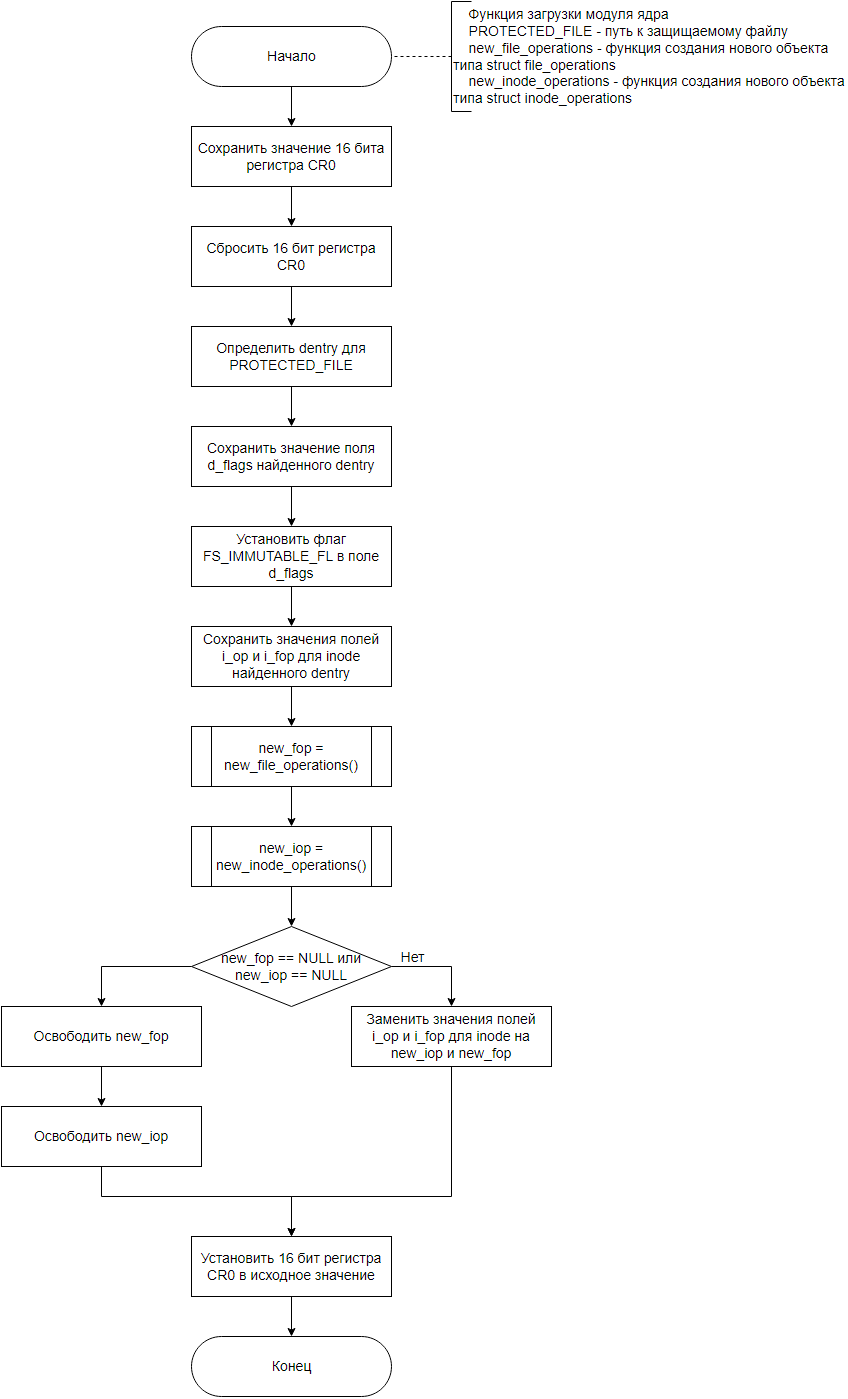
\includegraphics[width=150mm]{img/module_init.png}
	\caption{Схема алгоритма функции загрузки модуля ядра}
	\label{fig:module-init}
\end{figure}

\begin{figure}[h]
	\centering
	\captionsetup{justification=centering}
	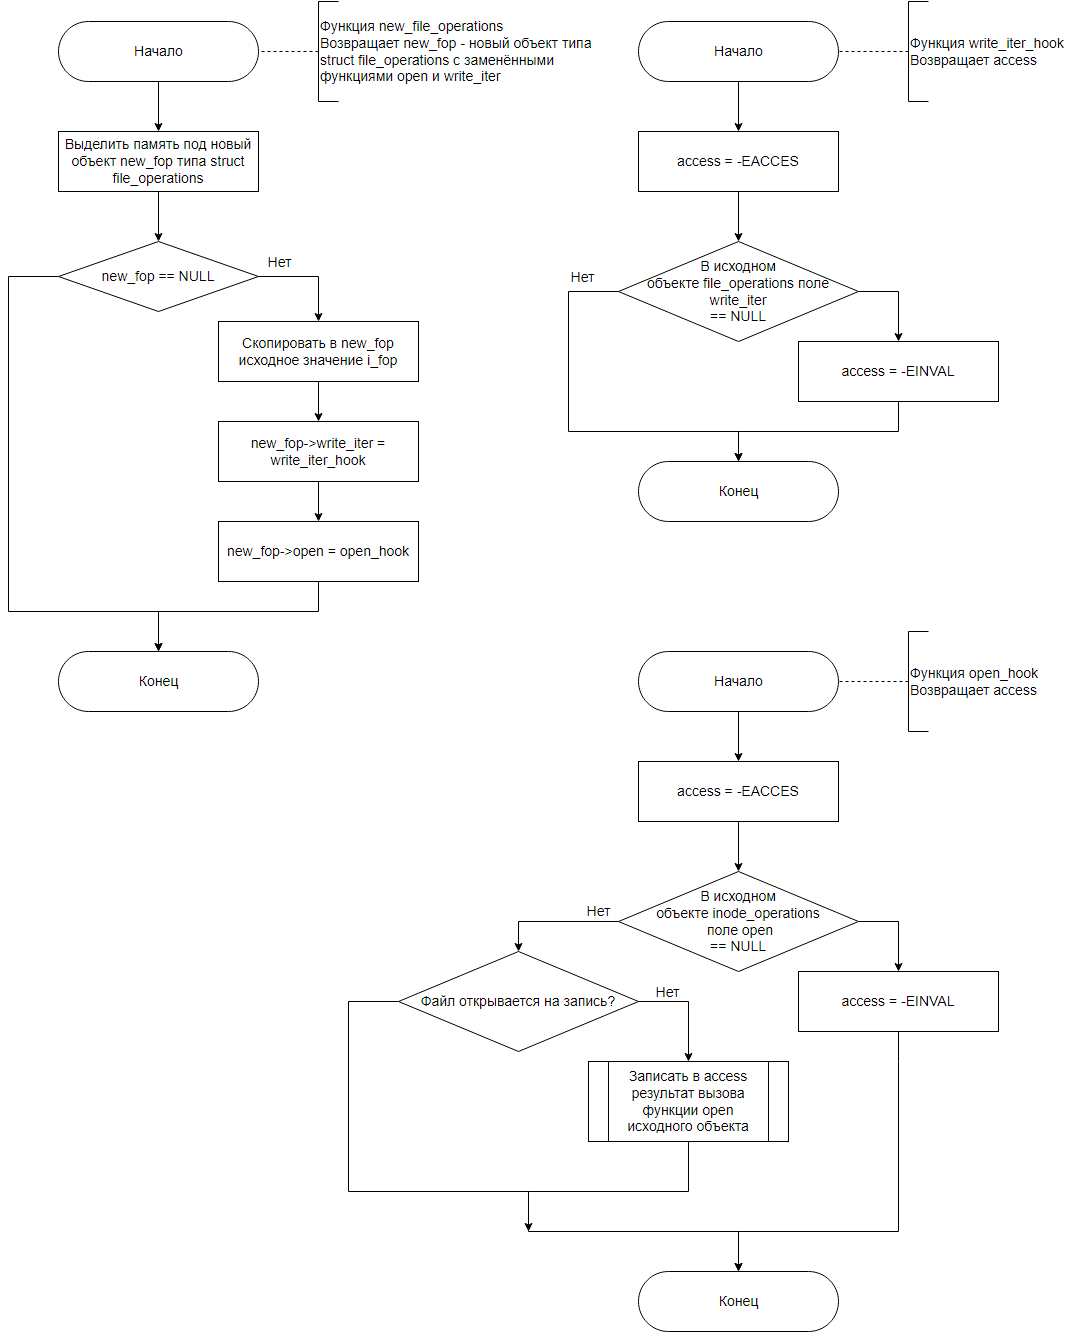
\includegraphics[width=170mm]{img/new_file_operations.png}
	\caption{Схемы алгоритмов создания нового объекта file\_operations и функций write\_iter\_hook и open\_hook}
	\label{fig:new-file-operations}
\end{figure}

\begin{figure}[h]
	\centering
	\captionsetup{justification=centering}
	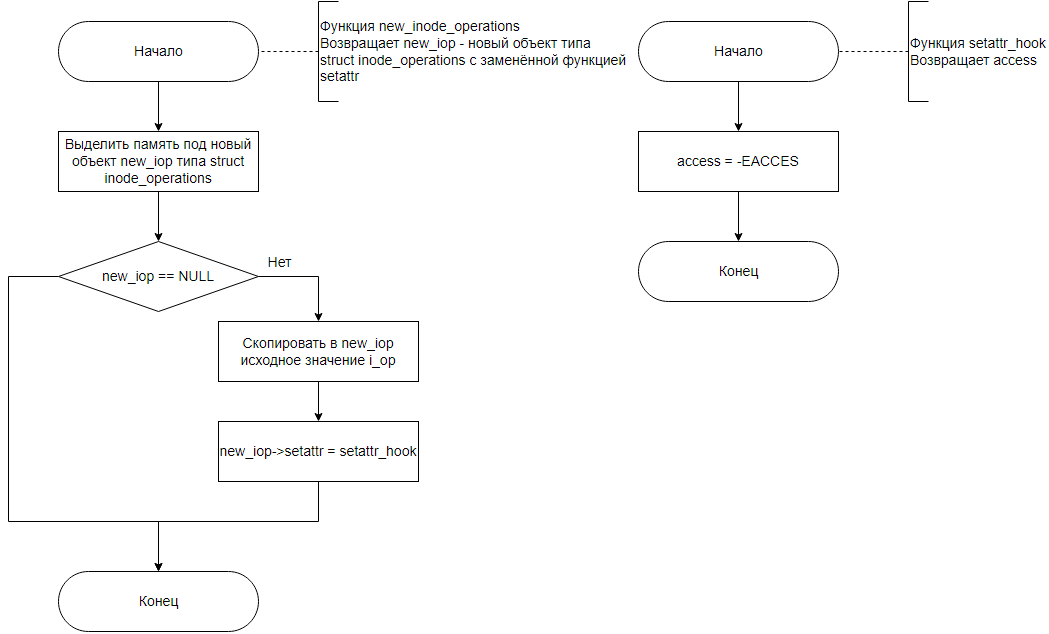
\includegraphics[width=170mm]{img/new_inode_operations.png}
	\caption{Схемы алгоритма создания нового объекта inode\_operations и функциии setattr\_hook}
	\label{fig:new-inode-operations}
\end{figure}

\begin{figure}[h]
	\centering
	\captionsetup{justification=centering}
	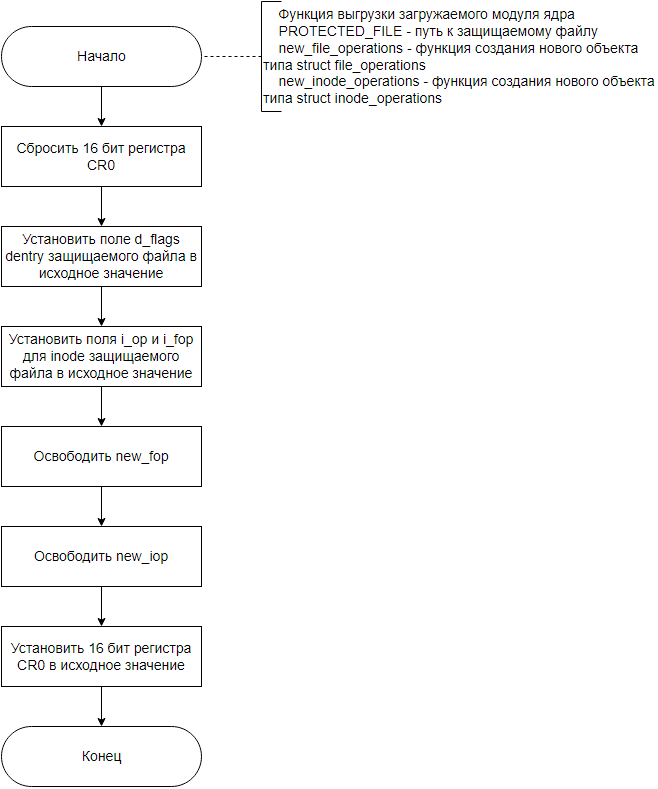
\includegraphics[width=170mm]{img/module_exit.png}
	\caption{Схема алгоритма выгрузки загружаемого модуля}
	\label{fig:module-exit}
\end{figure}


%\subsection*{Вывод}
%
%В данном разделе  была рассмотрена спроектированная база данных, соответствующая выбранной в  аналитической части СУБД, приведена диаграмма базы данных, рассмотрены сценарии создания таблиц БД и ролевой модели для управления доступом к таблицам, а также приведена диаграмма классов приложения и разобран основной используемый паттерн проектирования REST.

